\documentclass{article}
\usepackage{amsmath}
\usepackage{graphicx} % Required for inserting images

\title{Direction Estimation from Stereo XY Cardoid Microphones}
\author{Alex Grant}
\date{December 2023}

\begin{document}

\maketitle

\section{Introduction}
Consider microphones with cardoid response
\begin{equation*}
    f(\theta) = 2\alpha(1-\cos\theta)
\end{equation*}

\begin{figure}
    \centering
    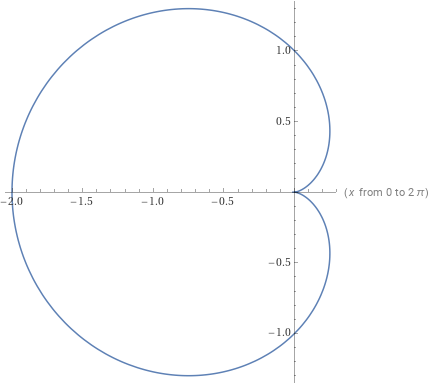
\includegraphics[width=0.5\linewidth]{cardoid.png}
    \caption{Cardoid with $\alpha=1$}
    \label{fig:cardoid}
\end{figure}

With two cardoid microphones arranged in an XY configuration and an angle of arrival $\theta$ (measured clockwise from the negative x-axis), the received power $P_L$ and $P_R$ for the left and right channels respectively are
\begin{align*}
    P_L &= 2\beta(1-\cos(\theta-\pi/4)) \\
    P_R &= 2\beta(1-\cos(\theta+\pi/4))
\end{align*}
where the $\pm \pi/4$ accounts for the 90 degree offset between the two microphones, and $\beta$ lumps the parameter $\alpha$ together with the unknown source signal strength.

Define the ratio
\begin{equation}
    \rho = \frac{P_L}{P_R} = \frac{(1-\cos(\theta-\pi/4))}{(1-\cos(\theta+\pi/4))}
\end{equation}
then direction finding can be performed by solving this equation for $\theta$, given the measurement $\rho$.

In practice solving for $\rho$ or $1/\rho$ can be performed to avoid ill-conditioned systems.

\end{document}
